% vim:ft=tex
% rubber: module xelatex

\subsection{Stereo matching}
\label{sec:stereo}
We have implemented dynamic programming based stereo matching using the methods
described by \citet{realtimestereo}. The output of the stereo matching is a
disparity map for each of the left and right images; the disparity map is a grey
scale image with black (or 0) signifying the lowest disparity, and white (or
255) signifying the maximum disparity. The disparity map is built using a
dynamic programming matrix for each scan line in the image; in the simplest
case, the process is as follows (for each scan line):

\begin{enumerate}
\item Create the dynamic programming matrix, $A$, with width and height both
  equal to the length of the scan line (i.e. the width of the images).
  Initialise the top-left corner to 0.

\item Step through the matrix, calculating $A[i,j] = \operator{min}(A[i-1,j],
  A[i,j-1], A[i-1,j-1])  +  \operator{diff}(imageL[i], imageR[j])$ where $diff$
  gets the difference between the image pixel values in the current scan line.

\item Calculate the path of minimal cost through the matrix $A$, starting in the
  bottom right corner, and moving from there to the adjacent position with the
  minimum value, i.e. $\operator{min}(A[i-1,j], A[i,j-1], A[i-1,j-1])$. Fill the
  disparity map with the appropriate value ($DisparityMapL[i,y]=j-i$,
  $DisparityMap[j,y]=i-j$).
\end{enumerate}

After having built up the disparity maps for the entire image (i.e. after doing
the above for all scan lines), go through them and normalise the values to the
range $[0,255]$, or, alternatively multiply the matrices by a user configurable
factor.

In addition to the simple version of the disparity mapping algorithm described
above, we have implemented the following (optional) modifications, in order to
improve the quality of the matching:

\begin{enumerate}
\item It is possible to assign an additional bonus or penalty to moving
  diagonally in the dynamic programming matrix, depending on whether we want
  smooth or spiky (very disparate) images respectively.

\item The choices for each scan line can be modified by those for the previous
  scan line, reducing error by ``suggesting'' ways to conform.

\item A median filter can be applied to the stereo images before building the
  disparity map, to get rid of noise.

\item It is possible to go through the dynamic programming matrix not only from
  the bottom-right to top-left corner, but also from top-left to bottom-right,
  and then choose the least-weight path overall. This helps reduce the cases
  where one of them goes horribly off the 'best' path because it, intuitively,
  followed the lowest-weight path into a dead end.

\item The running time can be improved by selecting a maximum disparity bound,
  $b$. The ``path of least resistance'' is never allowed to go outside this
  disparity bound because we set $A[i,j]$ to a vast positive value if $i > b$ or
  $j > b$.
\end{enumerate}


%%% Leaving this out for now...
% One improvement we didn't implement: line skipping. (In that version, at
% thebeginning, every n’th horizontal line is calculated to find bounding space
% for possible disparities in between.)


\subsubsection{Testing of stereo matching}

\begin{figure}[h]
  \centering
  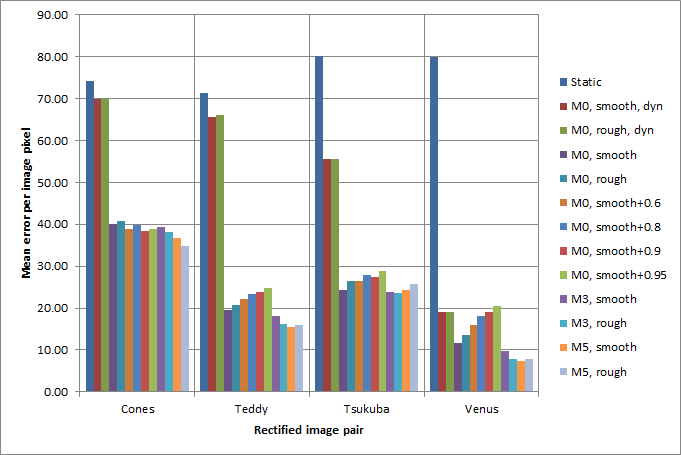
\includegraphics[width=0.8\textwidth]{Stereo-left-report}
  \caption[Results of dynamic programming (left image)]{Results of dynamic
    programming for the \emph{left} image, using various parameters. Resulting
    depth maps are compared to the canonical depth maps to obtain discrepancies
    (quantities of error). Each coloured column in the chart is a different
    parameterisation, as tested on one of the four images. `Static' is the
    baseline difference between the canonical depth map and a image with
    randomised values. `M0' indicates a median filter was not used in
    preprocessing. `M3' and `M5' indicate median filters of size 3 and 5
    respectively. `rough' indicates scanlines did not influence each other.
    `smooth' indicates each scanline was influenced by the one previous, by 0.5
    by default or by the amount given. `dyn' indicates the depth map was created
    by stretching the disparities to the full [0...255] range, instead of
    multiplying by the recommended value for each particular image.}
  \label{fig:stereo-left}
\end{figure}

\begin{figure}[h]
  \centering
  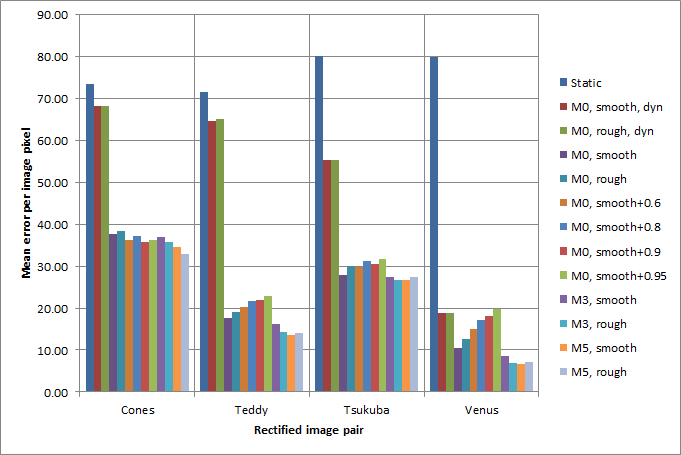
\includegraphics[width=0.8\textwidth]{Stereo-right-report}
  \caption[Results of dynamic programming (left image)]{Results of dynamic
    programming for the \emph{right} image, using various parameters. Resulting
    depth maps are compared to the canonical depth maps to obtain discrepancies
    (quantities of error). Each coloured column in the chart is a different
    parameterisation, as tested on one of the four images. `Static' is the
    baseline difference between the canonical depth map and a image with
    randomised values. `M0' indicates a median filter was not used in
    preprocessing. `M3' and `M5' indicate median filters of size 3 and 5
    respectively. `rough' indicates scanlines did not influence each other.
    `smooth' indicates each scanline was influenced by the one previous, by 0.5
    by default or by the amount given. `dyn' indicates the depth map was created
    by stretching the disparities to the full [0...255] range, instead of
    multiplying by the recommended value for each particular image.}
  \label{fig:stereo-right}
\end{figure}

